% Beamer slide template prepared by Tom Clark <tom.clark@op.ac.nz>
% Otago Polytechnic
% Dec 2012

\documentclass[10pt]{beamer}
\usetheme{CambridgeUS}
\usepackage{graphicx}
\usepackage{fancyvrb}

\newcommand\codeHighlight[1]{\textcolor[rgb]{1,0,0}{\textbf{#1}}}

\title{A Quick Overview of IPv6}

\author[IN715]{Networks Three}
\institute[Otago Polytechnic]{
  Otago Polytechnic \\
  Dunedin, New Zealand \\
}
\date{}
\begin{document}

%----------- titlepage ----------------------------------------------%
\begin{frame}[plain]
  \titlepage
\end{frame}



%----------- slide --------------------------------------------------%
\begin{frame}
  \frametitle{OSI Model}

 \begin{itemize}
  \item Application
  \item Presentaion
  \item Session
  \item Transport
  \item \textbf{Network}
  \item Data Link
  \item Physical
 \end{itemize}

\end{frame}

%----------- slide --------------------------------------------------%
\begin{frame}
  \frametitle{IPv4}

 \begin{itemize}
  \item IPv4 was released in 1980\footnote{RFC 760} - 1981\footnote{RFC 791}.
  \item It has been tremendously successful and will continue to be used for some time.
  \item It has some problems:
    \begin{itemize}
      \item address exhaustion
      \item complicated routing
      \item poor support for security, QoS
    \end{itemize}
 \end{itemize}

\end{frame}


%----------- slide --------------------------------------------------%
\begin{frame}
  \frametitle{A new protocol was needed}

 \begin{itemize}
  \item By the early 1990s it was clear that we needed a new protocol
  \item In 1992-1993, the IETF began looking into a version of IP.
  \item Relevant RFCs began to come out in 1996.
 \end{itemize}

\end{frame}


%----------- slide --------------------------------------------------%
\begin{frame}
  \frametitle{Some features of IPv6}

 \begin{itemize}
  \item Larger address space
  \item Simplified headers
  \item Hierachical addressing and routing
  \item Improved device autoconfiguration
  \item IPSec
 \end{itemize}

\end{frame}


%----------- slide --------------------------------------------------%
\begin{frame}
  \frametitle{IPv6 addresses}

 \begin{itemize}
  \item IPv6 addressed are 128 bits long.
  \item The first 64 bits are used to identify the network.
  \item The second 64 bits are used for the host.
  \item Example:
        2001:0DB8:AC10:FE01:0000:0000:0000:01A6 \\
        \hspace{15mm}2001:DB8:AC10:FE01::1A6
 \end{itemize}


\end{frame}


%----------- slide --------------------------------------------------%
\begin{frame}
  \frametitle{Address types}

 \begin{itemize}
  \item Unicast
        \begin{itemize}
          \item Global
          \item Link-Local
        \end{itemize}
  \item Multicast
  \item Anycast
  \item N.B.: No broadcast 
 \end{itemize}

\end{frame}


%----------- slide --------------------------------------------------%
\begin{frame}
  \frametitle{Address autoconfiguration}

 \begin{itemize}
  \item Manual configuration and DHCP are still available for IPv6
  \item Very briefly, autoconfiguration works like this:
      \begin{enumerate}
        \item a device determines its link-local address
        \item it sends \emph{router solicitaion} messages
        \item it receives \emph{router advertisements} in response
        \item from these the device determines its \emph{network prefix}
        \item it appends its 64 bit interface id to produce its address
      \end{enumerate}
 \end{itemize}

\end{frame}



%----------- slide --------------------------------------------------%
\begin{frame}
  \frametitle{EUI-64}

 \begin{itemize}
  \item An IPv6 interface typically uses EUI-64 to obtain its interface ID.
  \item Basically, we take the 48 bit MAC address and stretch it out to 64 bits.
  \item Example:
     \begin{enumerate}
       \item Start with a MAC address:  39:A7:97:07:CB:D0
       \item Insert FFFE into the middle:  39:A7:97:FF:FE:07:CB:D0
       \item Set the seventh\footnote{The universal-local bit} to 1:  3B:A7:97:FF:FE:07:CB:D0
     \end{enumerate}
 \end{itemize}

\end{frame}



%----------- slide --------------------------------------------------%
\begin{frame}
  \frametitle{Simplified Routing}
   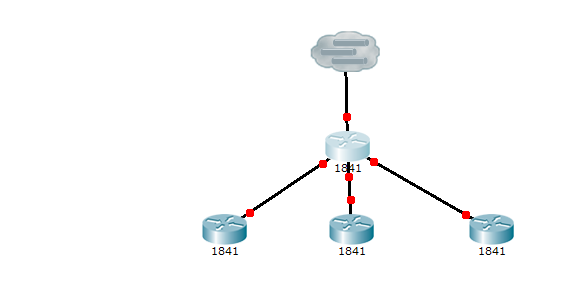
\includegraphics[scale=0.5]{nw.png}

\end{frame}

\end{document}
